\documentclass[12pt, a4paper]{report}
\usepackage[top=3cm,left=3cm,right=2cm,bottom=2cm]{geometry}
\linespread{1.3}
\setlength{\parindent}{1.25cm}
\usepackage{indentfirst}
\usepackage[utf8]{inputenc}
\usepackage[brazil]{babel}
\usepackage{amsmath}
\usepackage{amsthm}
\usepackage{amsfonts}
\usepackage{amssymb}
\usepackage{graphicx}
\usepackage{color}
\usepackage{multicol}
\usepackage[normalem]{ulem}
\usepackage{wrapfig}
\usepackage{caption}
\usepackage{fancybox}
\usepackage[pdfstartview=FitH]{hyperref}
\usepackage{subfigure}
\usepackage{algorithm}
\usepackage{algpseudocode}
\usepackage{float}
\usepackage{multirow}
\usepackage{siunitx}
\usepackage{rotating}
\usepackage{booktabs}

\graphicspath{{Figuras/}}

\renewcommand{\theenumii}{\alph{enumii}}
\DeclareMathOperator{\sen}{sen}
\DeclareMathOperator{\tg}{tg}
\DeclareMathOperator{\arctg}{arctg}
\DeclareMathOperator{\cotg}{cotg}
\DeclareMathOperator{\agm}{agm}

\newtheorem{thm}{Teorema}[section]
\newtheorem{dfn}{Definição}[section]
\newtheorem{prob}{Problema}[section]
\newtheorem{cor}{Corolário}[section]
\newtheorem{prop}{Proposição}[section]
\newtheorem{lem}{Lema} [section]

\newcounter{contar}

% Variáveis do projeto
\newcommand{\nomeUniversidade}{Universidade Federal da Bahia}
\newcommand{\nomeInstituto}{Instituto de Computação}
\newcommand{\nomeCurso}{Interação Humano-Computador}
\newcommand{\nomeProfessor}{Prof. Igor Sobral}
\newcommand{\nomeGrupo}{\sc{\large{Antoniel Magalhães (antoniels@ufba.br)}} \\
\sc{\large{André Costa (andre.lino@ufba.br)}} \\
\sc{\large{João Leahy (joao.leahy.ufba.br)}} \\
\sc{\large{Luis Felipe (luis.sena@ufba.br)}} \\
\sc{\large{Koichi Filho (koichifilho@ufba.br)}}
}
\newcommand{\titulo}{\sc{\Large{Projeto Prático Final: Sistema de Gestão de Monitorias (SIGA-M) \\ ETAPA 2 - SÍNTESE}}}

\begin{document}

% Capa
\pagestyle{empty}
\begin{center}

\includegraphics[height=2.5cm]{UFBA.jpg}
\hspace{2cm}
\end{center}

\begin{center}
\sc{\large{\nomeUniversidade}} \\
\sc{\large{\nomeInstituto}} \\
\sc{\small{\nomeCurso}} \\

\vspace{4cm}

\titulo

\vspace{4.5cm}

\nomeGrupo

\vspace{5.5cm}

\textbf{Salvador - Bahia} \\
1º de julho de 2025
\end{center}

% Folha de rosto
\newpage
\begin{center}
\titulo

\vspace{4cm}

\nomeGrupo
\end{center}

\vspace{4cm}

\begin{flushright}
\begin{minipage}{8.6cm}
Etapa 2 do projeto prático final apresentado ao professor \nomeProfessor\ 
como método avaliativo da disciplina \nomeCurso.
\end{minipage}
\end{flushright}
 
\vspace{8cm}

\begin{center}
\textbf{Salvador - Bahia} \\
1º de julho de 2025
\end{center}

% Índice
\newpage
\tableofcontents
\thispagestyle{empty}
\newpage
\setcounter{page}{1}
\pagestyle{plain}

\chapter{Etapa 2: Síntese (Intervenção)}
\label{ch:sintese}

Esta etapa apresenta a proposta de intervenção sob a forma de um protótipo interativo do sistema SIGA-M, focando no fluxo essencial entre coordenador e professor para o ciclo de criação e aprovação de projetos de monitoria.

\section{Modelo de Interação}

O modelo de interação apresenta o fluxo simplificado de navegação entre as telas principais do sistema, concentrando-se no processo fundamental de criação, submissão e aprovação de projetos de monitoria. O desenvolvimento partiu de um protótipo de baixa fidelidade (Figura \ref{fig:excalidraw}) que estabeleceu as bases para o design final.

\begin{figure}[H]
\centering
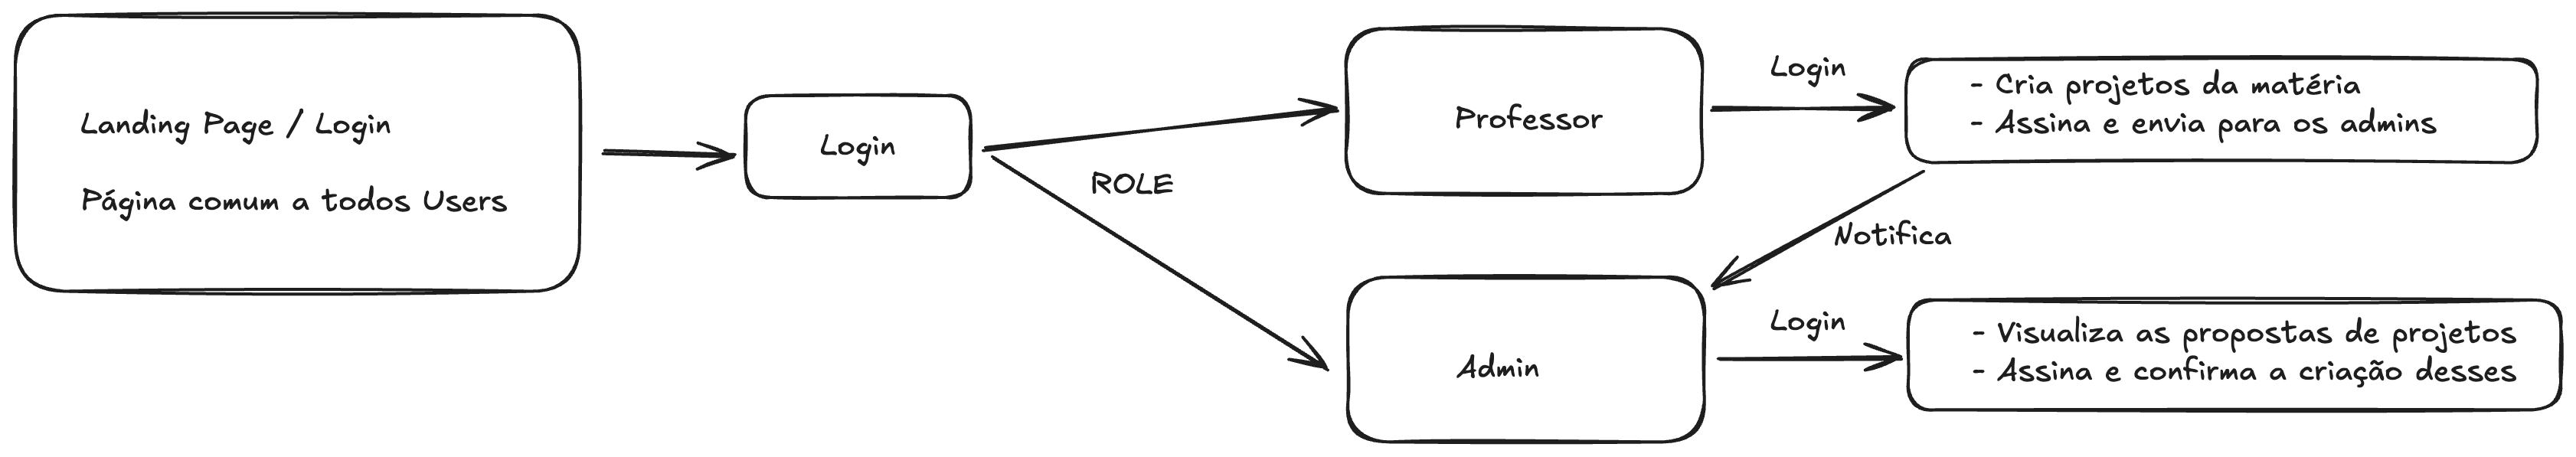
\includegraphics[width=0.8\textwidth]{figma/excalidraw-design.png}
\caption{Protótipo de baixa fidelidade - Base inicial do design}
\label{fig:excalidraw}
\end{figure}

O fluxo principal simplificado segue duas jornadas essenciais:
\begin{itemize}
    \item \textbf{Jornada do Professor}: Login → Criar/Editar Projeto → Enviar Projeto
    \item \textbf{Jornada do Administrador}: Login → Visualizar Projetos → Aprovar/Assinar → Iniciar Processo de Bolsa
\end{itemize}

\subsection{Fluxo de Interação Principal}

O modelo de interação foi otimizado para os dois perfis principais:

\subsubsection{Fluxo do Professor}
\begin{enumerate}
    \item \textbf{Login}: Autenticação via credenciais institucionais
    \item \textbf{Dashboard}: Visualização de projetos existentes ou opção de criar novo
    \item \textbf{Criação de Projeto}: Formulário com dados pré-preenchidos quando disponíveis
    \item \textbf{Revisão}: Verificação das informações do projeto
    \item \textbf{Envio}: Submissão do projeto para aprovação do coordenador
    \item \textbf{Confirmação}: Feedback visual de sucesso no envio
\end{enumerate}

\subsubsection{Fluxo do Administrador (Coordenador)}
\begin{enumerate}
    \item \textbf{Login}: Acesso com perfil administrativo
    \item \textbf{Dashboard}: Visão geral de todos os projetos submetidos
    \item \textbf{Análise}: Revisão detalhada de cada projeto
    \item \textbf{Aprovação}: Assinatura digital e aprovação do projeto
    \item \textbf{Inicialização}: Ativação do processo de bolsa de monitoria
    \item \textbf{Notificação}: Sistema notifica automaticamente os envolvidos
\end{enumerate}

\subsection{Tratamento de Erros e Recuperação}

O sistema implementa mecanismos essenciais de tratamento de erros:

\begin{itemize}
    \item \textbf{Validação de Login}: Feedback claro para credenciais inválidas
    \item \textbf{Salvamento Automático}: Prevenção de perda de dados durante criação de projetos
    \item \textbf{Confirmações}: Diálogos de confirmação antes de ações críticas
    \item \textbf{Navegação Segura}: Sempre com opção de voltar sem perder progresso
\end{itemize}

\section{Link de Acesso ao Protótipo}

O protótipo interativo está disponível na plataforma Figma através do seguinte link:

\url{https://www.figma.com/design/meTbBaQdqBHlvtzBEb9ehF/Sistema-de-Monitoria-IC?node-id=1-2&p=f}

O protótipo permite a simulação completa do fluxo simplificado professor-coordenador, possibilitando a navegação interativa pelas funcionalidades essenciais do sistema.

\section{Telas e Decisões de Projeto}

As capturas de tela do protótipo e as justificativas das decisões de design são apresentadas a seguir, focando no fluxo principal:

\subsection{Tela de Login}

\begin{figure}[H]
\centering
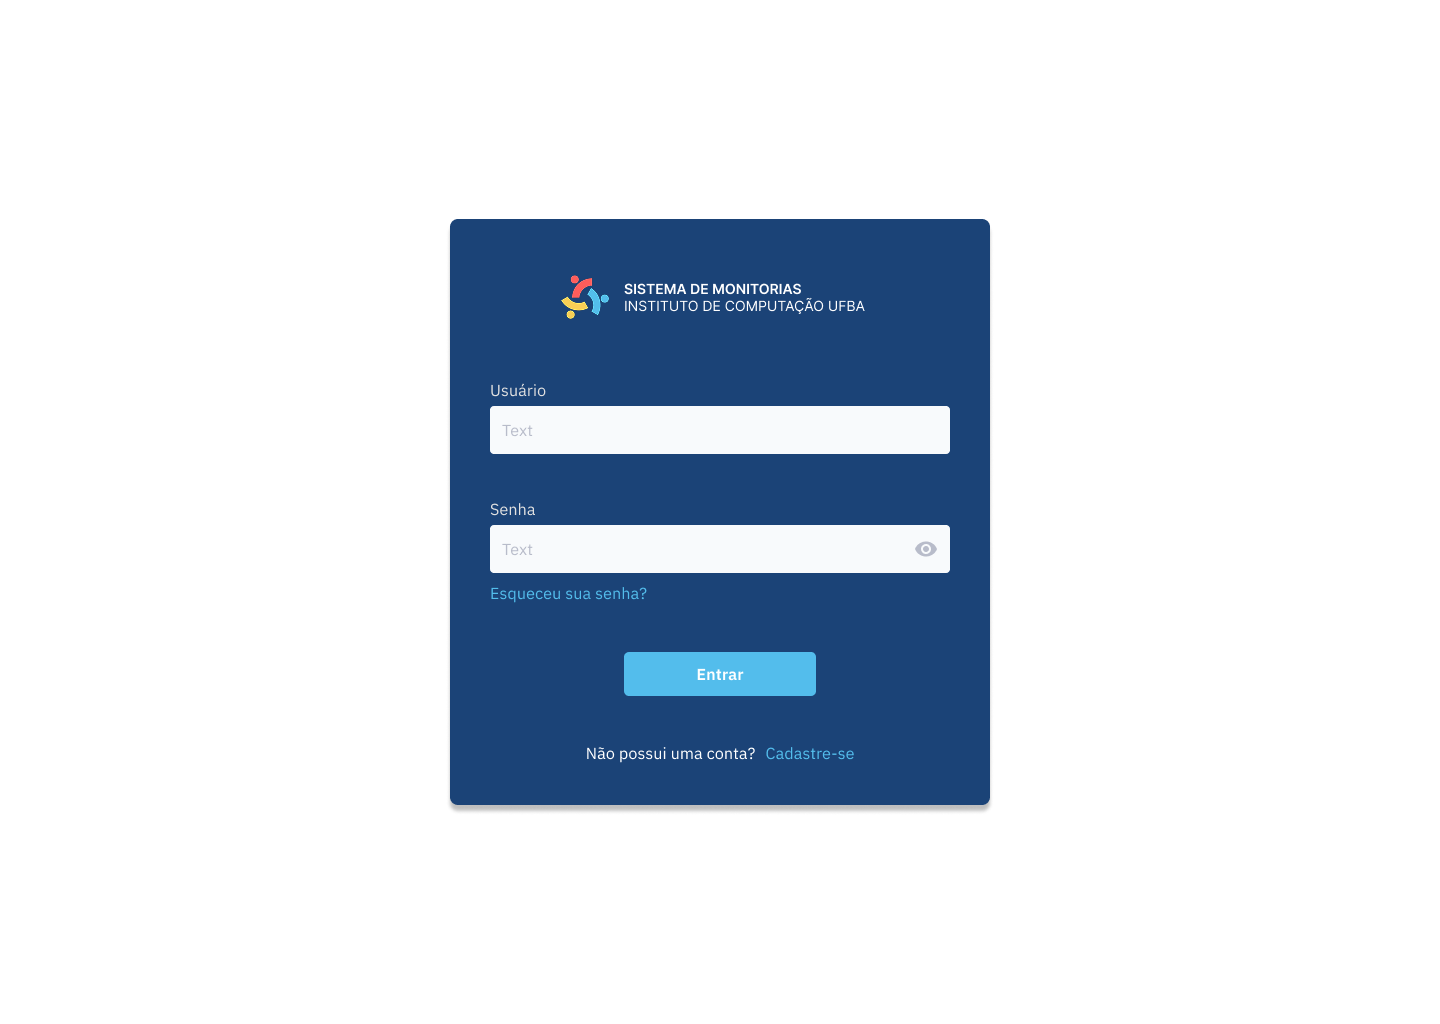
\includegraphics[width=0.8\textwidth]{figma/Login.png}
\caption{Tela de Login do Sistema SIGA-M}
\label{fig:login}
\end{figure}

\textbf{Decisões de Design}:
\begin{itemize}
    \item \textbf{Identidade Visual}: Utilização das cores institucionais da UFBA (azul) para criar familiaridade
    \item \textbf{Simplicidade}: Layout limpo com foco nos campos essenciais
    \item \textbf{Diferenciação de Perfis}: Login único com identificação automática do tipo de usuário
    \item \textbf{Segurança Visual}: Campo de senha com opção de visualização
\end{itemize}

\subsection{Formulário de Criação de Projeto}

\begin{figure}[H]
\centering
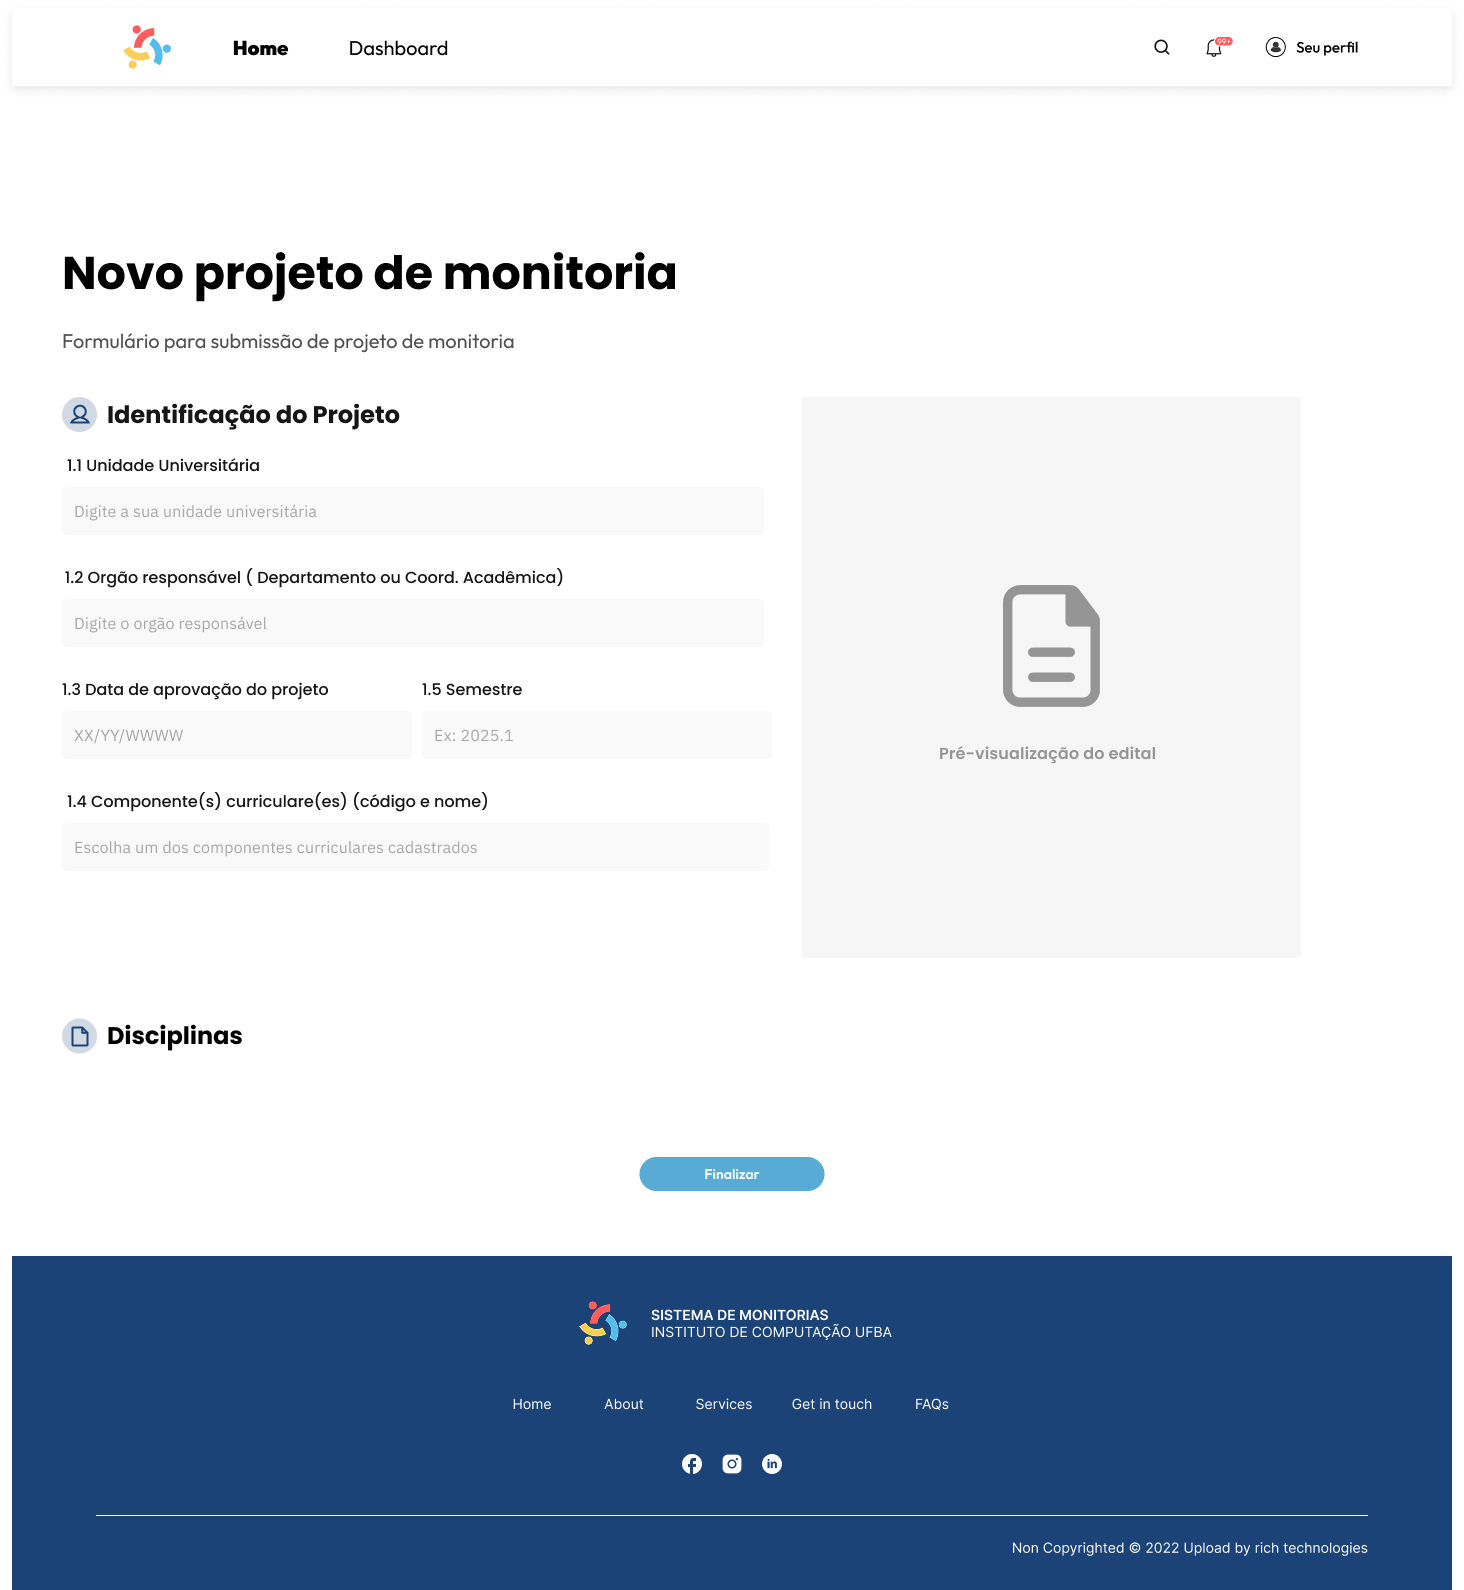
\includegraphics[width=0.9\textwidth]{figma/projeto-monitoria.png}
\caption{Interface de Criação de Projeto de Monitoria}
\label{fig:projeto-monitoria}
\end{figure}

\textbf{Decisões de Design}:
\begin{itemize}
    \item \textbf{Formulário Estruturado}: Campos organizados logicamente seguindo o fluxo do documento oficial
    \item \textbf{Pré-preenchimento Inteligente}: Dados do professor e histórico carregados automaticamente
    \item \textbf{Validação em Tempo Real}: Indicadores visuais de campos obrigatórios e validados
    \item \textbf{Ações Claras}: Botões de "Salvar Rascunho" e "Enviar para Aprovação" bem posicionados
    \item \textbf{Navegação Contextual}: Breadcrumb indicando posição no processo
\end{itemize}

\subsection{Dashboard do Coordenador}

\begin{figure}[H]
\centering
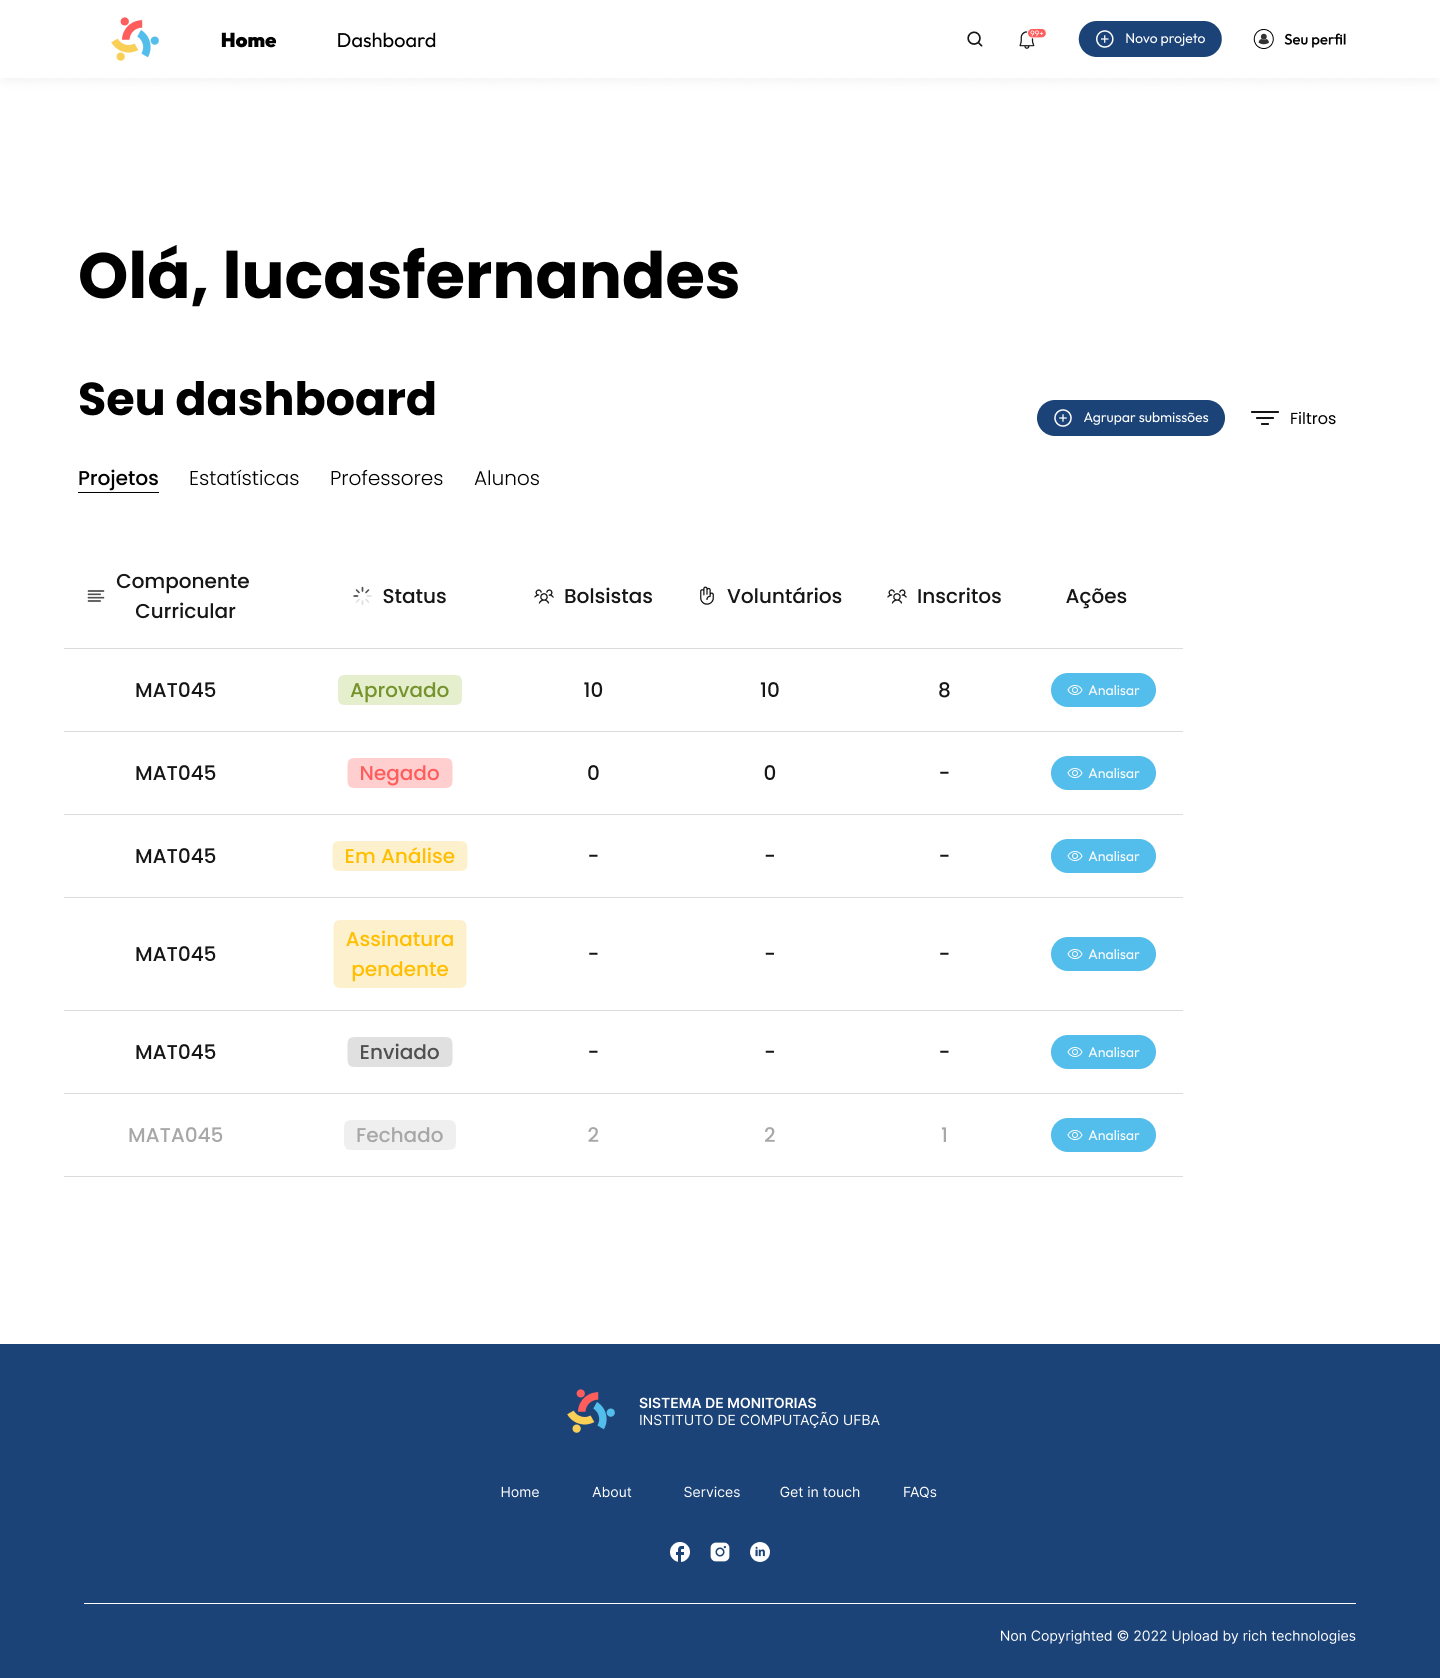
\includegraphics[width=0.8\textwidth]{figma/Dashboard_coodenador.png}
\caption{Dashboard do Coordenador - Visão de Projetos}
\label{fig:dashboard}
\end{figure}

\textbf{Decisões de Design}:
\begin{itemize}
    \item \textbf{Visão Consolidada}: Lista de todos os projetos com status visual claro
    \item \textbf{Filtros Rápidos}: Opções para filtrar por status (pendente, aprovado, em análise)
    \item \textbf{Ações em Lote}: Possibilidade de aprovar múltiplos projetos
    \item \textbf{Informações Essenciais}: Exibição de dados críticos (professor, disciplina, data de submissão)
    \item \textbf{Acesso Rápido}: Links diretos para visualizar detalhes de cada projeto
\end{itemize}

\subsection{Paleta de Cores}

\begin{figure}[H]
\centering
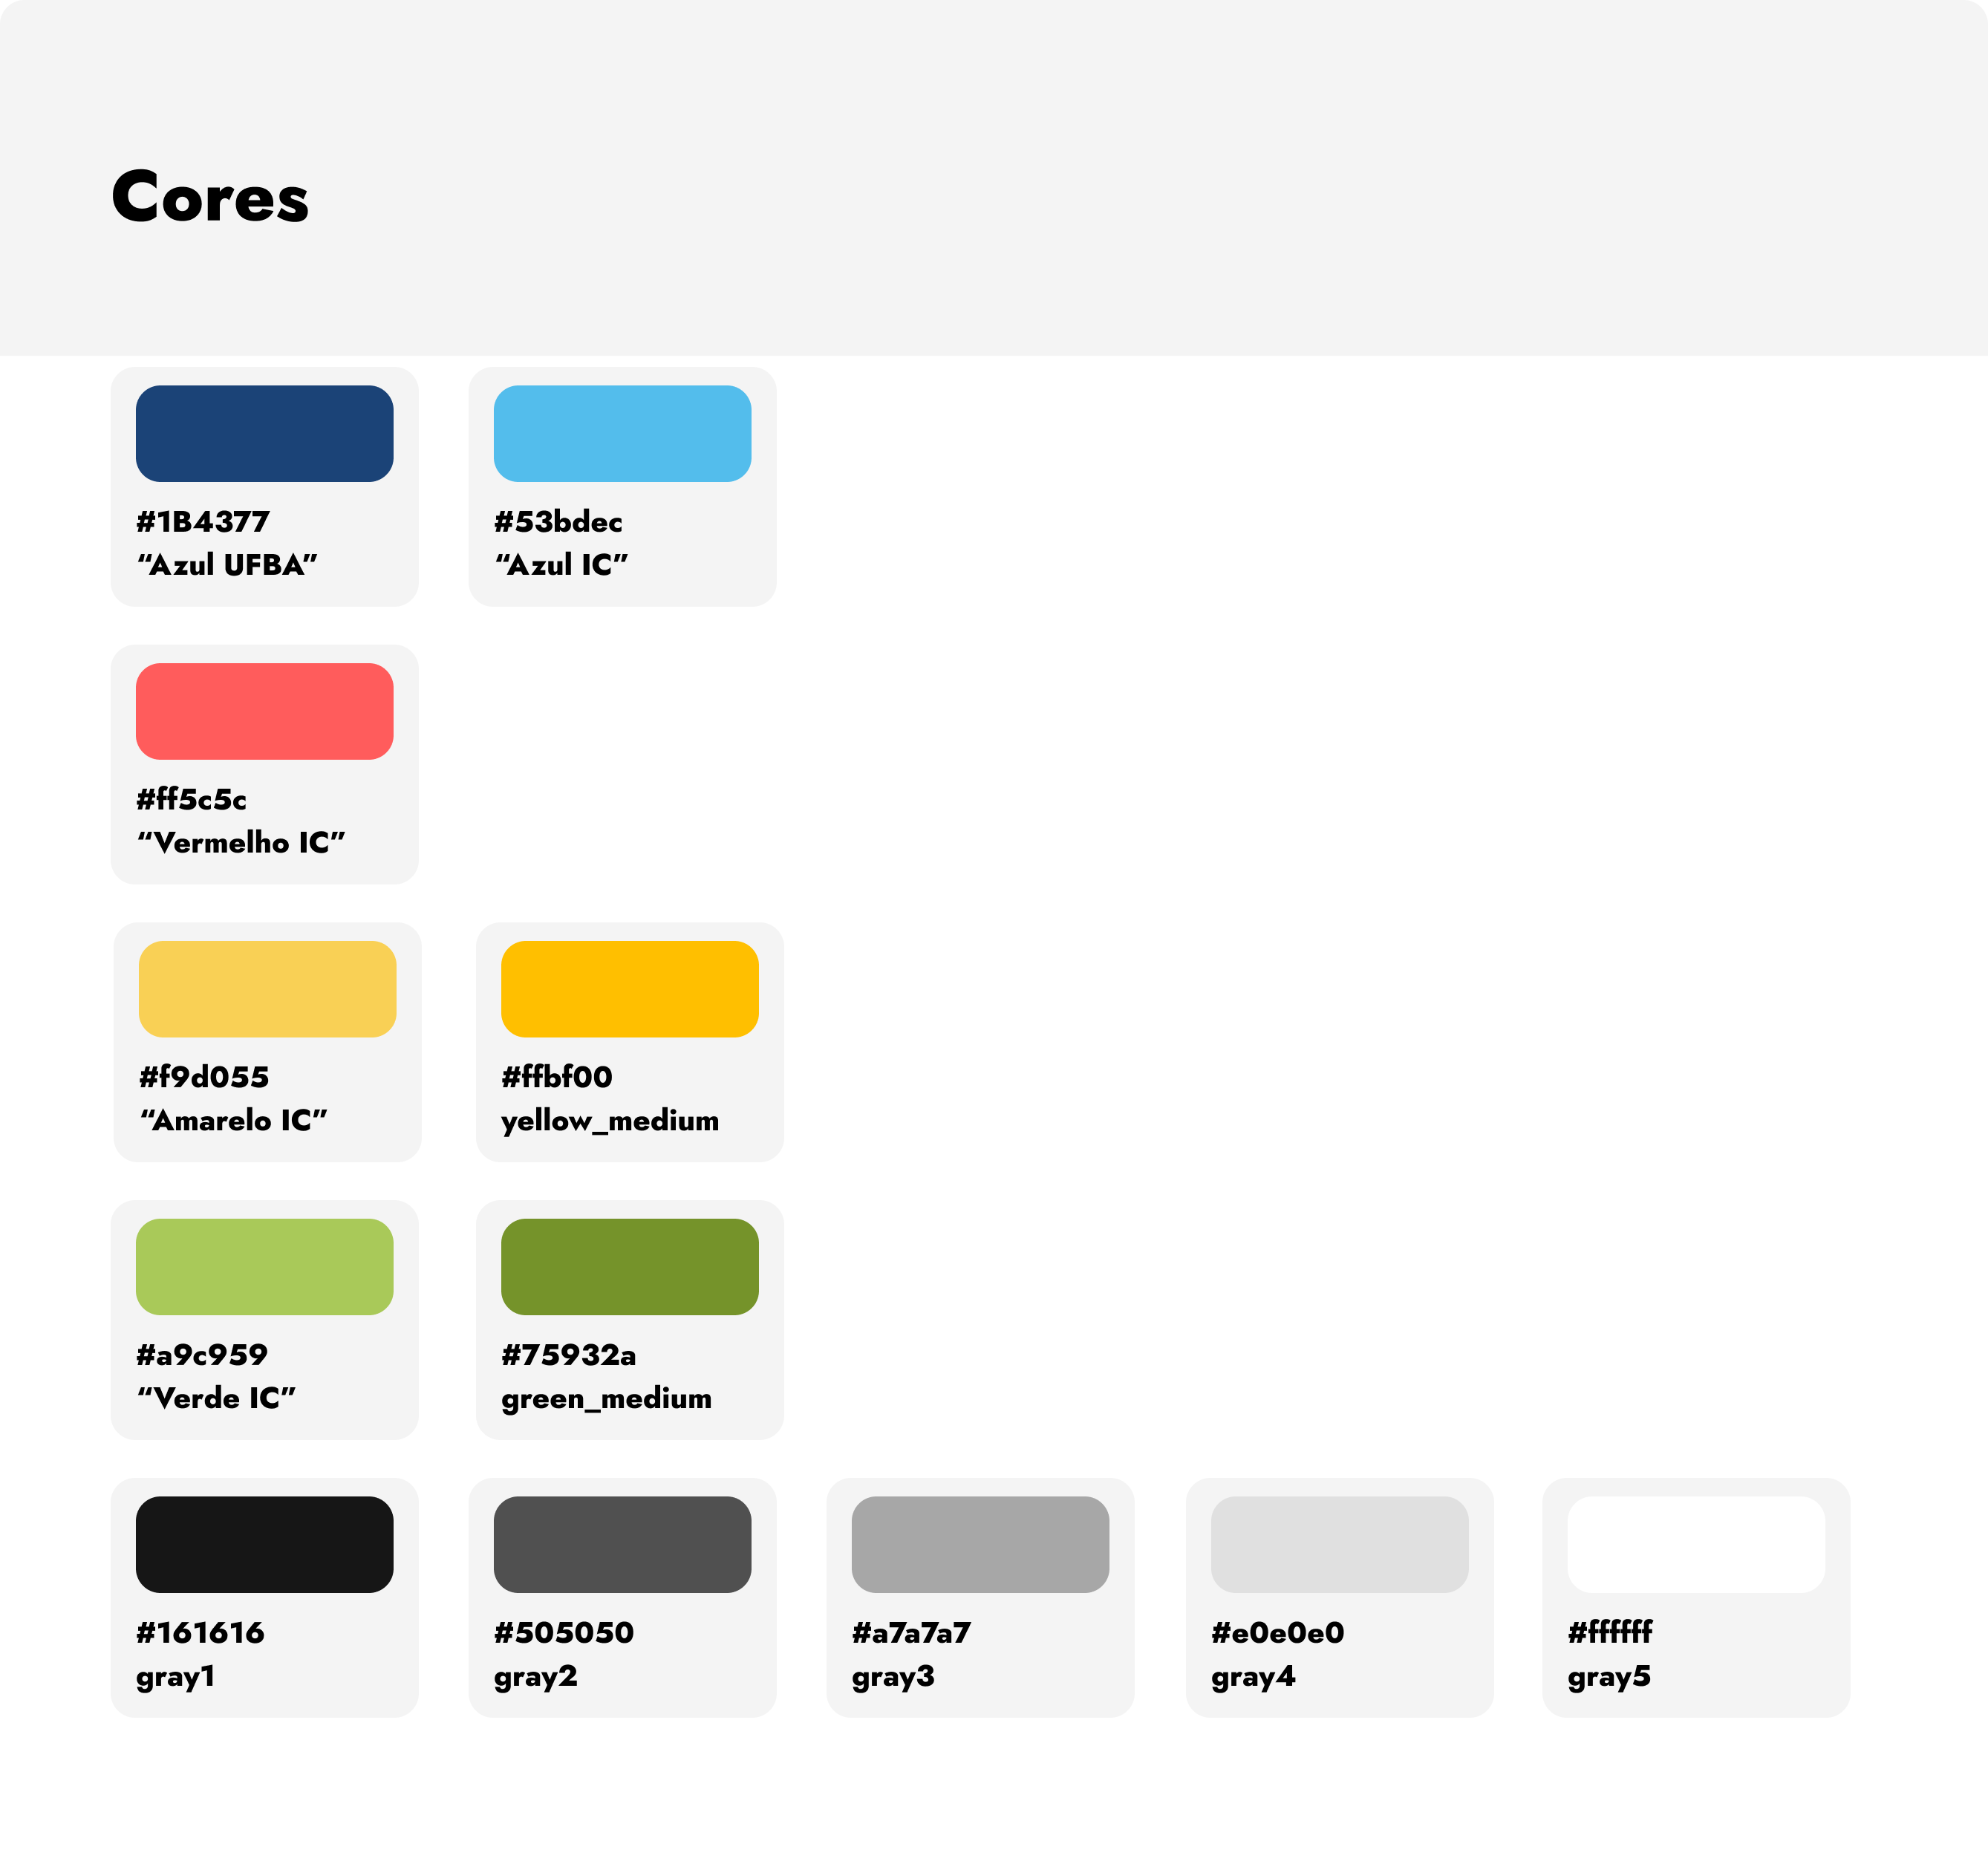
\includegraphics[width=0.8\textwidth]{figma/Cores.png}
\caption{Paleta de Cores Utilizada no Sistema}
\label{fig:cores}
\end{figure}

\textbf{Justificativa da Paleta}:
\begin{itemize}
    \item \textbf{Azul Institucional}: Cor primária da UFBA mantida para consistência
    \item \textbf{Verde de Aprovação}: Para indicar projetos aprovados e ações positivas
    \item \textbf{Amarelo de Pendência}: Para projetos aguardando análise
    \item \textbf{Cinzas Neutros}: Para elementos de interface e textos secundários
    \item \textbf{Alto Contraste}: Garantia de acessibilidade visual
\end{itemize}

\subsection{Tipografia}

\begin{figure}[H]
\centering
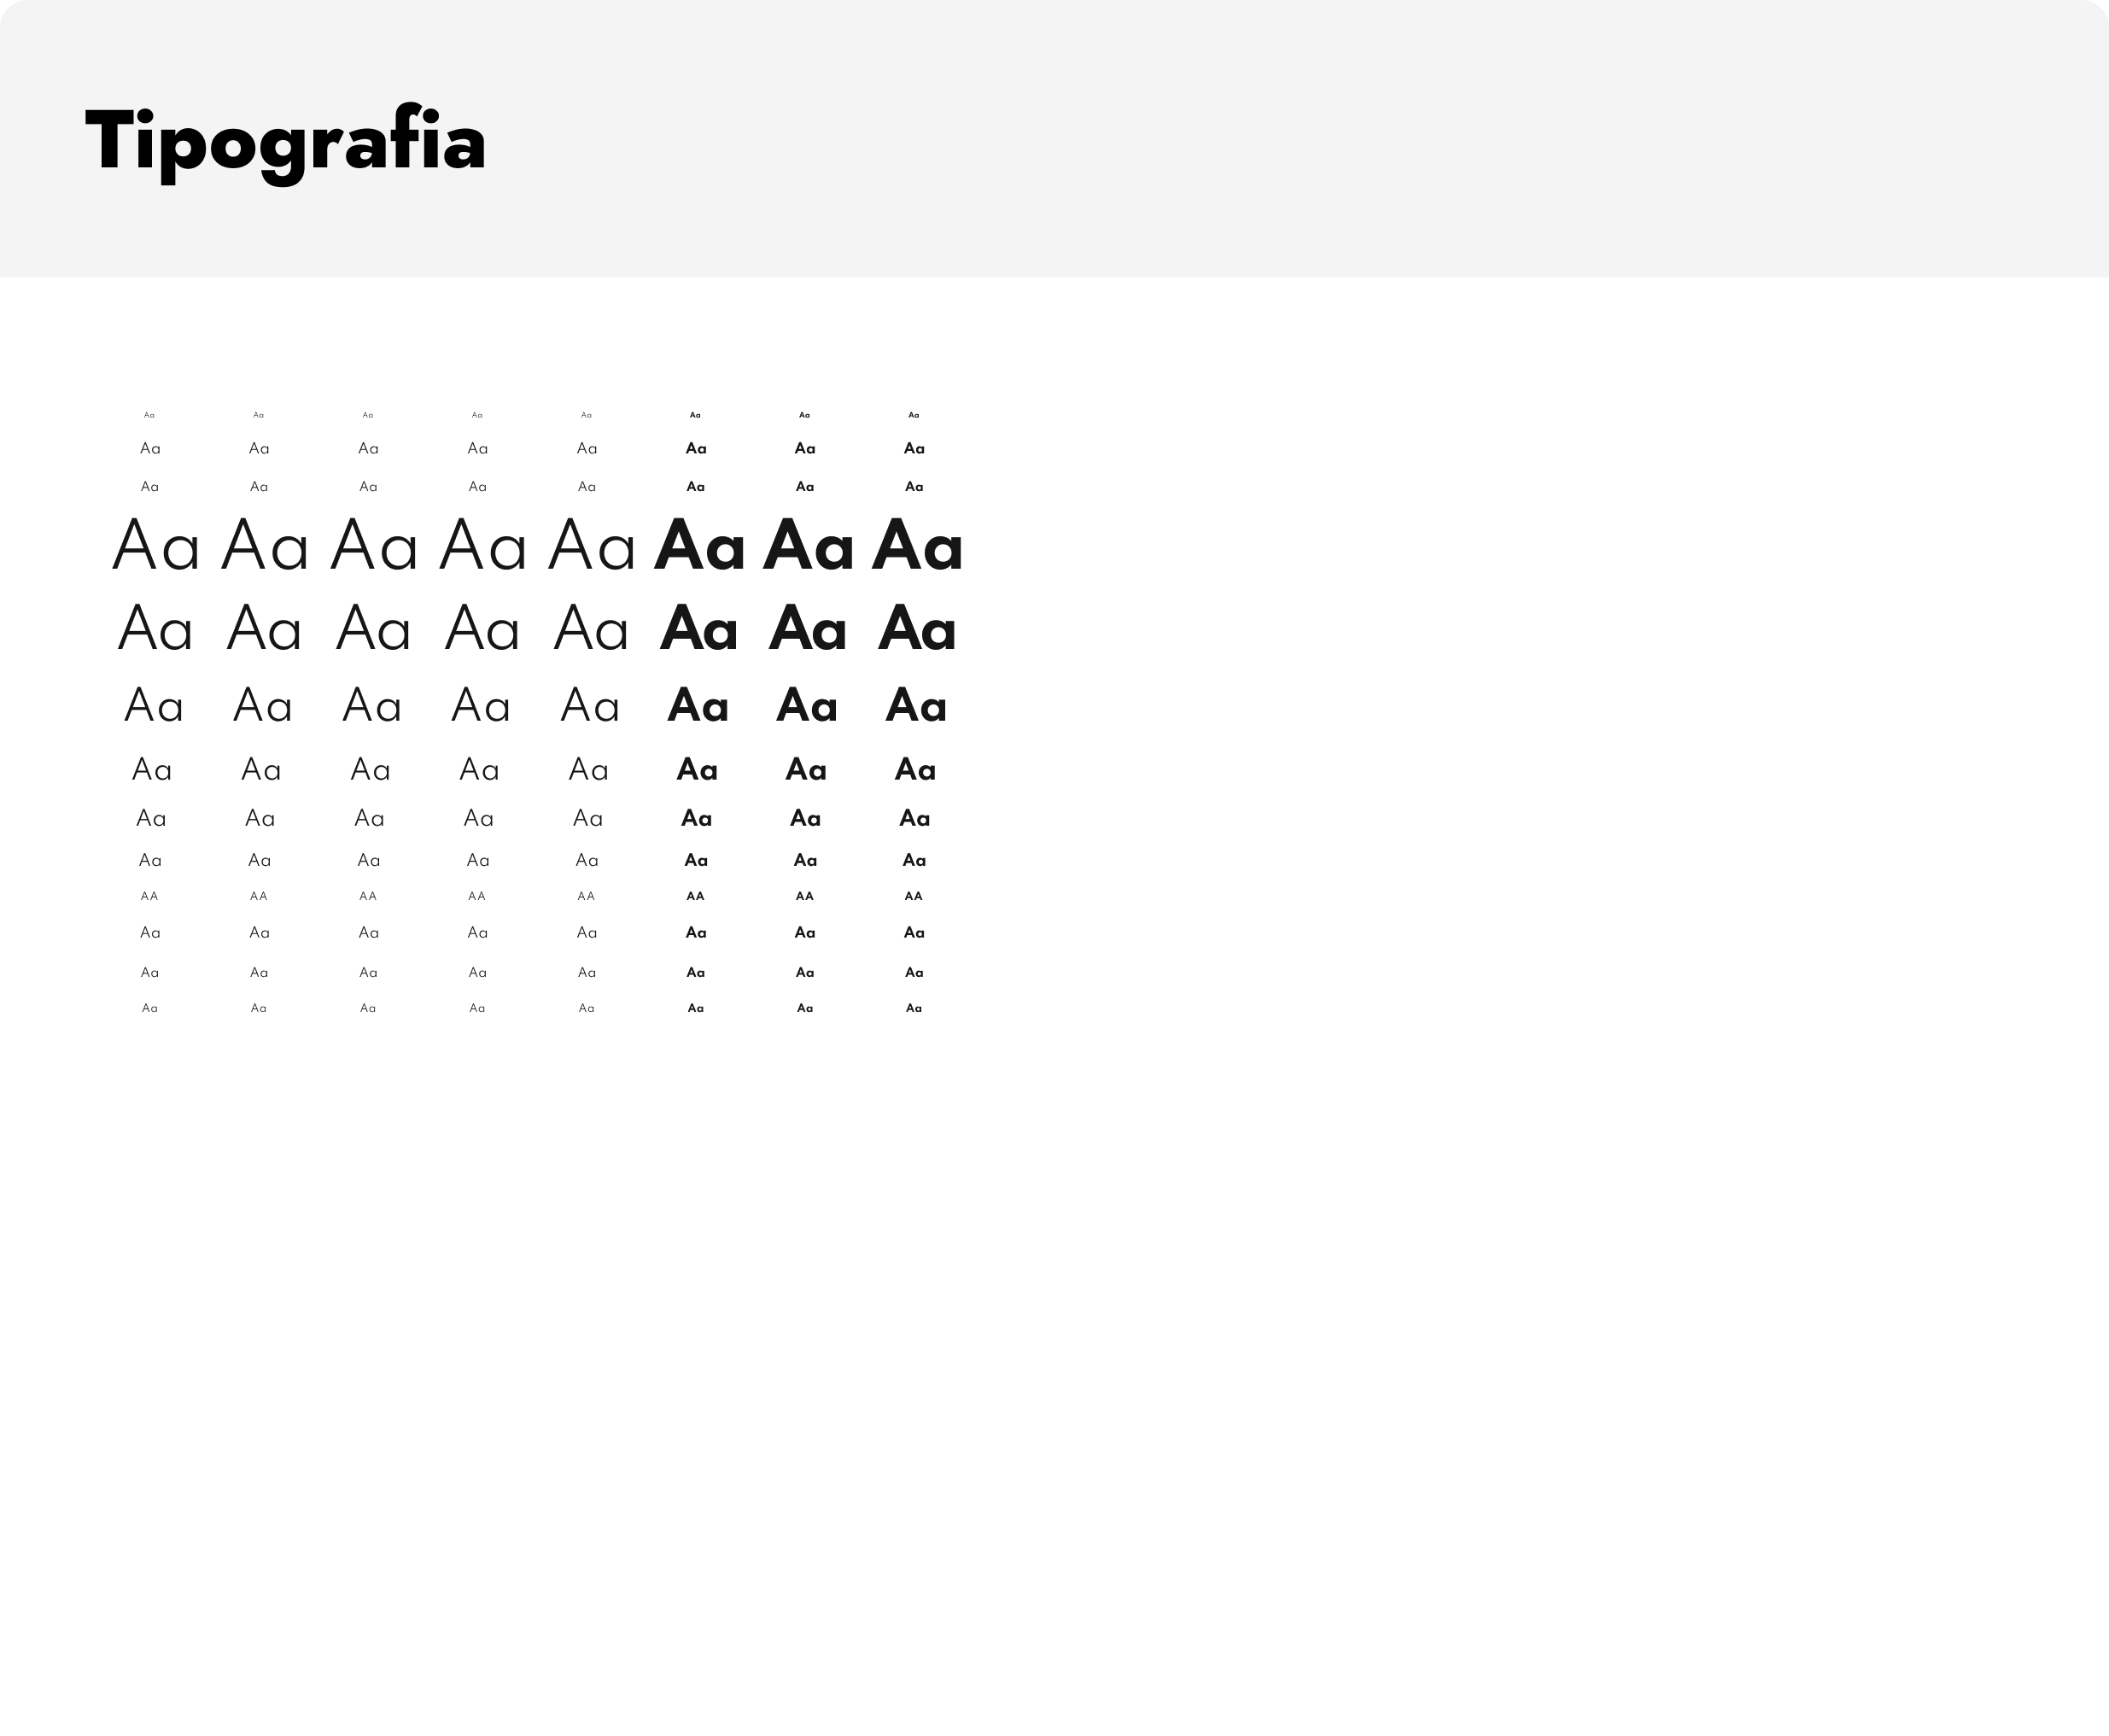
\includegraphics[width=0.8\textwidth]{figma/Tipografia.png}
\caption{Sistema Tipográfico do SIGA-M}
\label{fig:tipografia}
\end{figure}

\textbf{Decisões Tipográficas}:
\begin{itemize}
    \item \textbf{Hierarquia Clara}: Títulos, subtítulos e corpo de texto bem diferenciados
    \item \textbf{Legibilidade}: Fontes sans-serif para leitura em tela
    \item \textbf{Consistência}: Mesmo sistema tipográfico em todo o protótipo
    \item \textbf{Tamanhos Adequados}: Mínimo de 14px para corpo de texto
\end{itemize}

\section{Princípios de Design Aplicados}

\subsection{Foco na Tarefa Principal}

O protótipo foi desenvolvido com foco absoluto no fluxo crítico:

\begin{itemize}
    \item \textbf{Eliminação de Complexidade}: Apenas funcionalidades essenciais implementadas
    \item \textbf{Caminho Direto}: Mínimo de cliques para completar tarefas principais
    \item \textbf{Clareza de Propósito}: Cada tela tem objetivo único e claro
    \item \textbf{Feedback Imediato}: Confirmações visuais para cada ação importante
\end{itemize}

\subsection{Usabilidade Simplificada}

Considerações especiais para o contexto acadêmico:

\begin{itemize}
    \item \textbf{Familiaridade}: Interface similar a outros sistemas da UFBA
    \item \textbf{Linguagem Clara}: Terminologia alinhada com documentos oficiais
    \item \textbf{Processo Guiado}: Fluxo linear sem ramificações desnecessárias
    \item \textbf{Recuperação Fácil}: Sempre possível corrigir erros sem perder trabalho
\end{itemize}

\end{document} 